% !TEX program = xelatex
\documentclass[aspectratio=169, 10pt]{beamer}

% Use default theme with custom colors (avoids metropolis font dependency)
\usetheme{default}
\usecolortheme{dove}
\usefonttheme{professionalfonts}
\setbeamertemplate{navigation symbols}{}
\setbeamertemplate{footline}[frame number]

% Packages
\usepackage{booktabs}
\usepackage{tikz}
\usetikzlibrary{arrows.meta, positioning, calc, fit, backgrounds}
\usepackage{listings}
\usepackage{xcolor}
\usepackage{graphicx}
\usepackage{amsmath, amssymb}

% Lean 4 syntax highlighting
\lstdefinelanguage{Lean4}{
  keywords={theorem, lemma, def, abbrev, private, noncomputable, section, namespace,
    end, where, open, import, variable, set_option, by, intro, apply, exact,
    have, obtain, let, fun, match, if, then, else, do, return, sorry,
    simp, rw, ring, norm_num, ext, constructor, cases, induction, refine,
    calc, show, change, conv, at, with, in, deriving, instance, class,
    structure, inductive, example},
  keywordstyle=\color{violet}\bfseries,
  sensitive=true,
  comment=[l]{--},
  morecomment=[s]{/-}{-/},
  commentstyle=\color{gray}\itshape,
  stringstyle=\color{teal},
  morestring=[b]",
  literate=
    {->}{{$\to$}}2
    {<-}{{$\leftarrow$}}2
    {forall}{{$\forall$}}1
    {exists}{{$\exists$}}1
    {<=}{{$\leq$}}2
    {>=}{{$\geq$}}2
    {:=}{{$\,:=$}}2,
  basicstyle=\ttfamily\scriptsize,
  breaklines=true,
  showstringspaces=false,
  tabsize=2,
  frame=none,
  numbers=none,
}

\lstset{language=Lean4}

% NUS Official Colors
\definecolor{nus-orange}{RGB}{239, 124, 0}
\definecolor{nus-blue}{RGB}{0, 61, 124}
\definecolor{nus-orange-light}{RGB}{255, 224, 204}
\definecolor{nus-orange-mid}{RGB}{255, 163, 102}
% Supplementary colors
\definecolor{statblue}{RGB}{0, 61, 124}       % alias for nus-blue
\definecolor{statgreen}{RGB}{0, 150, 80}
\definecolor{statred}{RGB}{200, 50, 50}
\definecolor{statyellow}{RGB}{220, 160, 0}
\definecolor{statorange}{RGB}{239, 124, 0}    % alias for nus-orange
\definecolor{lightbg}{RGB}{245, 248, 252}

% NUS-styled beamer colors
\setbeamercolor{frametitle}{fg=white, bg=nus-blue}
\setbeamercolor{title}{fg=white, bg=nus-orange}
\setbeamercolor{alerted text}{fg=statred}
\setbeamercolor{block title}{fg=white, bg=nus-blue}
\setbeamercolor{block body}{bg=nus-blue!5}
\setbeamercolor{block title alerted}{fg=white, bg=statred}
\setbeamercolor{block body alerted}{bg=statred!5}
\setbeamercolor{block title example}{fg=white, bg=statgreen!80!black}
\setbeamercolor{block body example}{bg=statgreen!5}
\setbeamercolor{structure}{fg=nus-blue}
\setbeamercolor{itemize item}{fg=nus-orange}
\setbeamercolor{enumerate item}{fg=nus-orange}
\setbeamercolor{section in head/foot}{bg=nus-blue, fg=white}
\setbeamercolor{subsection in head/foot}{bg=nus-blue, fg=white}
\setbeamercolor{footline}{fg=nus-blue}

% NUS-styled footline with logo text
\setbeamertemplate{footline}{%
  \leavevmode%
  \hbox{%
    \begin{beamercolorbox}[wd=.4\paperwidth,ht=2.5ex,dp=1ex,left]{footline}%
      \hspace*{1em}{\scriptsize\color{nus-blue} National University of Singapore}%
    \end{beamercolorbox}%
    \begin{beamercolorbox}[wd=.6\paperwidth,ht=2.5ex,dp=1ex,right]{footline}%
      {\scriptsize\color{nus-blue}\insertframenumber{} / \inserttotalframenumber}\hspace*{1em}%
    \end{beamercolorbox}%
  }%
  \vskip0pt%
}

% Frametitle with orange accent bar
\setbeamertemplate{frametitle}{%
  \nointerlineskip%
  \begin{beamercolorbox}[wd=\paperwidth,ht=2.5ex,dp=1ex]{frametitle}%
    \hspace*{1em}\insertframetitle%
  \end{beamercolorbox}%
  \nointerlineskip%
  {\color{nus-orange}\rule{\paperwidth}{2pt}}%
}

% NUS Logo
\titlegraphic{
\includegraphics[height=1.8cm]{figures/nus_logo}}

% Metadata
\title{\textbf{StatLean}}
\subtitle{A Lean 4 Formalization of Statistics}
\author{Gan Tong}
\date{March 2026}
\institute{Department of Statistics and Data Science\\National University of Singapore}

\begin{document}

% ============================================================
% Slide 1: Title (NUS branded)
% ============================================================
\begin{frame}[plain]
\begin{tikzpicture}[remember picture, overlay]
  % Top orange bar
  \fill[nus-orange] (current page.north west) rectangle ([yshift=-0.4cm]current page.north east);
  % Bottom blue bar
  \fill[nus-blue] (current page.south west) rectangle ([yshift=0.6cm]current page.south east);
  \node[anchor=south east, inner sep=0pt] at ([xshift=-0.8cm, yshift=0.08cm]current page.south east)
    {\scriptsize\color{white} National University of Singapore};
\end{tikzpicture}
\titlepage
\end{frame}

% ============================================================
% Slide 2: Motivation
% ============================================================
\begin{frame}{Why Formalize Statistics?}

\begin{columns}[T]
\begin{column}{0.48\textwidth}
\textbf{The Problem}
\begin{itemize}
  \item In the LLM era, training on statistical proofs requires high-quality formal data
  \item Lean 4 + Mathlib provide a mature platform for mathematics
  \item But \textbf{no comprehensive statistics library} exists yet
\end{itemize}
\vspace{0.5em}
\textbf{Our Approach}
\begin{itemize}
  \item \textbf{AI-assisted formalization}: LLM-driven proof search with human guidance
  \item Build on \textbf{Mathlib} (measure theory, probability, analysis)
  \item \textbf{Automated curation}: verified lemmas auto-indexed into reusable library
\end{itemize}
\end{column}
\begin{column}{0.48\textwidth}
\textbf{Benefits}
\begin{enumerate}
  \item \textbf{Reusability}: proved lemmas compose into larger results
  \item \textbf{Discovery}: formalization reveals hidden structure and missing conditions
\end{enumerate}
\end{column}
\end{columns}

\end{frame}

% ============================================================
% Slide 3: Project Overview
% ============================================================
\begin{frame}{Project Overview}

\textbf{Tech Stack}
\begin{itemize}
  \item Lean 4.28 + Mathlib (latest)
  \item Lake build system
\end{itemize}

\vspace{0.8em}
\textbf{Scale}
\begin{center}
\begin{tabular}{rl}
  \toprule
  \textbf{45} & Lean source files \\
  \textbf{14,400+} & lines of Lean code \\
  \textbf{490+} & formal declarations \\
  \textbf{38} & fully verified modules (zero \texttt{sorry}) \\
  \textbf{6} & remaining \texttt{sorry} gaps \\
  \bottomrule
\end{tabular}
\end{center}

\vspace{0.3em}
{\small\color{statgreen} \texttt{lake build Statlean.Verified} $\to$ zero warnings}

\end{frame}

% ============================================================
% Slide 4: End-to-End Pipeline (moved before dependency map)
% ============================================================
\begin{frame}{End-to-End Formalization Pipeline}
\begin{center}
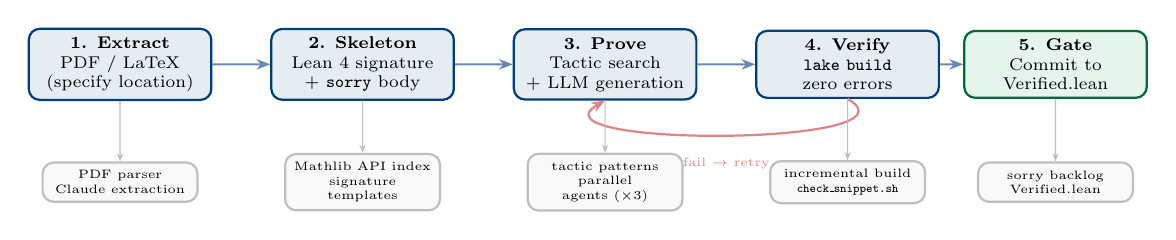
\begin{tikzpicture}[
  every node/.style={font=\scriptsize, rounded corners=4pt, thick, minimum height=0.8cm, align=center},
  phase/.style={draw=statblue, fill=statblue!10, text width=2.4cm},
  tool/.style={draw=gray!50, fill=gray!5, font=\tiny, text width=2.0cm, minimum height=0.5cm},
  output/.style={draw=statgreen!70!black, fill=statgreen!10, text width=2.4cm},
  arr/.style={-{Stealth[length=5pt]}, thick, statblue!60},
  darr/.style={-{Stealth[length=3pt]}, thin, gray!50},
  scale=0.88, transform shape
]
  % Main pipeline (horizontal)
  \node[phase] (pdf) at (0, 2)    {\textbf{1. Extract}\\PDF / LaTeX\\(specify location)};
  \node[phase] (skel) at (3.5, 2) {\textbf{2. Skeleton}\\Lean 4 signature\\+ \texttt{sorry} body};
  \node[phase] (prove) at (7, 2)  {\textbf{3. Prove}\\Tactic search\\+ LLM generation};
  \node[phase] (verify) at (10.5, 2) {\textbf{4. Verify}\\\texttt{lake build}\\zero errors};
  \node[output] (commit) at (13.5, 2) {\textbf{5. Gate}\\Commit to\\Verified.lean};

  \draw[arr] (pdf) -- (skel);
  \draw[arr] (skel) -- (prove);
  \draw[arr] (prove) -- (verify);
  \draw[arr] (verify) -- (commit);

  % Retry loop
  \draw[arr, statred!60] (verify.south) to[out=-30, in=-150]
    node[below, font=\tiny, draw=none, fill=none, text width=1.5cm] {fail $\to$ retry} (prove.south);

  % Tools below each phase
  \node[tool] (t1) at (0, 0.3)    {PDF parser\\Claude extraction};
  \node[tool] (t2) at (3.5, 0.3)  {Mathlib API index\\signature templates};
  \node[tool] (t3) at (7, 0.3)    {tactic patterns\\parallel agents ($\times$3)};
  \node[tool] (t4) at (10.5, 0.3) {incremental build\\\texttt{check\_snippet.sh}};
  \node[tool] (t5) at (13.5, 0.3) {sorry backlog\\Verified.lean};

  \draw[darr] (pdf) -- (t1);
  \draw[darr] (skel) -- (t2);
  \draw[darr] (prove) -- (t3);
  \draw[darr] (verify) -- (t4);
  \draw[darr] (commit) -- (t5);

\end{tikzpicture}
\end{center}

\vspace{0.3em}
\begin{columns}[T]
\begin{column}{0.48\textwidth}
\textbf{Input}: PDF/LaTeX with specified theorem location,\\
or direct text description of the theorem to formalize\\
\textbf{Output}: machine-verified Lean 4 proof
\end{column}
\begin{column}{0.48\textwidth}
\textbf{Automation}: Steps 1--4 driven by Claude Code\\
\textbf{Human}: review gate at Step 5, mathematical guidance
\end{column}
\end{columns}

\end{frame}

% ============================================================
% Slide 5: Skeleton Generation Detail
% ============================================================
\begin{frame}{Step 1--2: From Textbook to Lean Skeleton}

\begin{columns}[T]
\begin{column}{0.48\textwidth}
\textbf{Theorem Extraction}
\begin{enumerate}
  \item Parse PDF / LaTeX source
  \item Identify theorem statement, hypotheses, notation
  \item Map to Mathlib types and conventions
  \item Resolve ambiguity with textbook context
\end{enumerate}

\vspace{0.5em}
\textbf{Signature Design Principles}
\begin{itemize}
  \item Follow Mathlib conventions (universe-polymorphic, typeclass args)
  \item All conditions explicit (no ``clearly integrable'')
\end{itemize}
\end{column}
\begin{column}{0.48\textwidth}
\textbf{Mathlib API Search} (3-tier, mandatory)

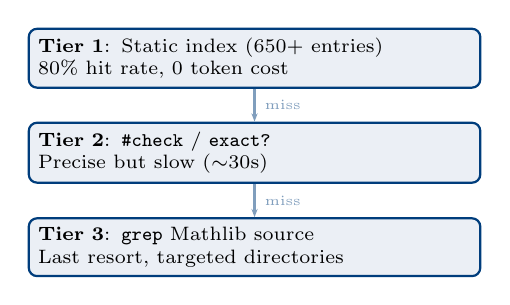
\begin{tikzpicture}[
  every node/.style={font=\scriptsize, rounded corners=3pt, thick, minimum height=0.6cm, align=left, text width=5.5cm},
  tier/.style={draw=statblue, fill=statblue!8},
  arr/.style={-{Stealth[length=3pt]}, thick, statblue!50},
]
  \node[tier] (l1) at (0, 3)   {\textbf{Tier 1}: Static index (650+ entries)\\80\% hit rate, 0 token cost};
  \node[tier] (l2) at (0, 1.8) {\textbf{Tier 2}: \texttt{\#check} / \texttt{exact?}\\Precise but slow ($\sim$30s)};
  \node[tier] (l3) at (0, 0.6) {\textbf{Tier 3}: \texttt{grep} Mathlib source\\Last resort, targeted directories};

  \draw[arr] (l1) -- node[right, font=\tiny, draw=none, fill=none, text width=0.8cm] {miss} (l2);
  \draw[arr] (l2) -- node[right, font=\tiny, draw=none, fill=none, text width=0.8cm] {miss} (l3);
\end{tikzpicture}

\vspace{0.5em}
{\small Avoids redundant Mathlib searches --- the biggest token cost in LLM-based proving.}
\end{column}
\end{columns}

\end{frame}

% ============================================================
% Slide 7: Prove + Verify Detail
% ============================================================
\begin{frame}{Step 3--4: Prove and Verify}

\begin{columns}[T]
\begin{column}{0.52\textwidth}
\textbf{Sorry DAG Scheduler}

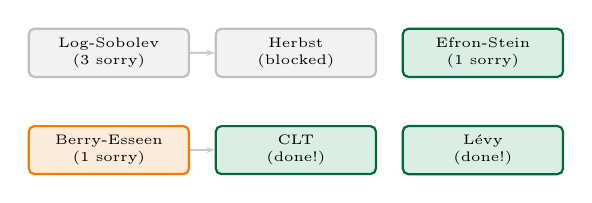
\begin{tikzpicture}[
  every node/.style={font=\tiny, rounded corners=2pt, thick, minimum height=0.45cm, align=center, text width=1.8cm},
  leaf/.style={draw=statgreen!70!black, fill=statgreen!15},
  blocked/.style={draw=gray!50, fill=gray!10},
  active/.style={draw=statorange, fill=statorange!15},
  arr/.style={-{Stealth[length=3pt]}, thick, gray!40},
  scale=0.95
]
  \node[blocked] (lsi) at (0, 2.5)    {Log-Sobolev\\(3 sorry)};
  \node[blocked] (herb) at (2.5, 2.5) {Herbst\\(blocked)};
  \node[leaf]    (ef)   at (5, 2.5)   {Efron-Stein\\(1 sorry)};
  \node[active]  (be)   at (0, 1.2)   {Berry-Esseen\\(1 sorry)};
  \node[leaf, draw=statgreen!70!black] (clt) at (2.5, 1.2) {CLT\\(done!)};
  \node[leaf, draw=statgreen!70!black] (levy) at (5, 1.2) {L\'{e}vy\\(done!)};

  \draw[arr] (lsi) -- (herb);
  \draw[arr] (be.east) -- (clt.west);
\end{tikzpicture}

\vspace{0.3em}
\begin{itemize}
  \item \textbf{Leaves first}: attack goals with no downstream dependencies
  \item \textbf{Skip blocked}: don't waste cycles on dependency chains
  \item \textbf{Parallel}: up to 3 agents on independent goals
\end{itemize}

\vspace{0.2em}
\textbf{Tactic Pattern Library}
\begin{itemize}
  \item Indexed by goal shape (e.g.\ ``$\int f\,d\mu = 0$'' $\to$ \texttt{integral\_condExp})
  \item Only verified patterns (\texttt{lake build} passed)
\end{itemize}
\end{column}
\begin{column}{0.45\textwidth}
\textbf{Verification Loop}

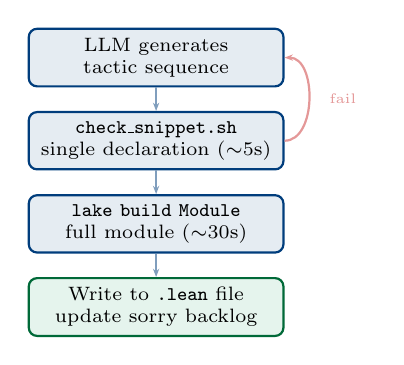
\begin{tikzpicture}[
  every node/.style={font=\scriptsize, rounded corners=3pt, thick, minimum height=0.55cm, align=center, text width=3.0cm},
  wfstep/.style={draw=statblue, fill=statblue!10},
  arr/.style={-{Stealth[length=3pt]}, thick, statblue!50},
  scale=0.88
]
  \node[wfstep] (g1) at (0, 4.2) {LLM generates\\tactic sequence};
  \node[wfstep] (g2) at (0, 3.0) {\texttt{check\_snippet.sh}\\single declaration ($\sim$5s)};
  \node[wfstep] (g3) at (0, 1.8) {\texttt{lake build Module}\\full module ($\sim$30s)};
  \node[wfstep, draw=statgreen!70!black, fill=statgreen!10] (g4) at (0, 0.6) {Write to \texttt{.lean} file\\update sorry backlog};

  \draw[arr] (g1) -- (g2);
  \draw[arr] (g2) -- (g3);
  \draw[arr] (g3) -- (g4);
  \draw[arr, statred!50] (g2.east) to[out=0, in=0]
    node[right, font=\tiny, text width=0.6cm, draw=none, fill=none] {fail} (g1.east);
\end{tikzpicture}

\vspace{0.3em}
\textbf{Key}: sub-lemmas written to disk \emph{immediately} after verification --- context exhaustion won't lose progress.
\end{column}
\end{columns}

\end{frame}

% ============================================================
% Slide 7b: Theorem Dependency Map (moved after Prove+Verify)
% ============================================================
\begin{frame}{Theorem Dependency Map}
\begin{center}
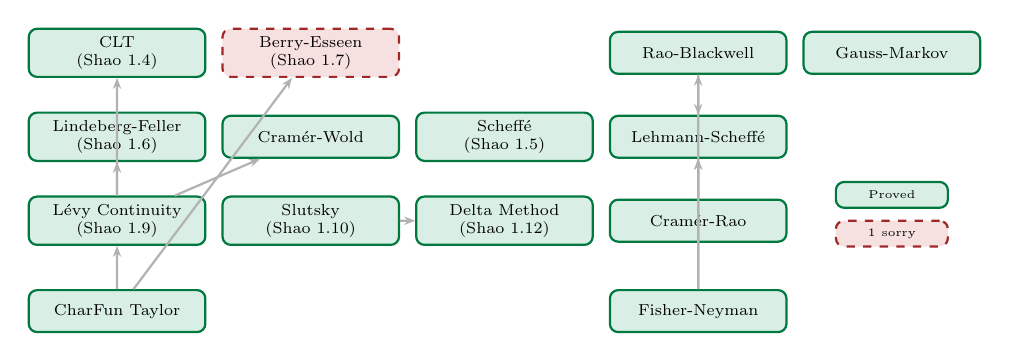
\begin{tikzpicture}[
  every node/.style={font=\scriptsize, rounded corners=3pt, minimum height=0.65cm, align=center, text width=2.5cm},
  proved/.style={draw=statgreen!80!black, fill=statgreen!15, thick},
  sorry/.style={draw=statred!80!black, fill=statred!15, thick, dashed},
  arr/.style={-{Stealth[length=4pt]}, thick, gray!60},
  scale=0.82, transform shape
]
  % Limit theorems column
  \node[proved] (clt)   at (0, 4)   {CLT\\(Shao 1.4)};
  \node[proved] (lf)    at (0, 2.7) {Lindeberg-Feller\\(Shao 1.6)};
  \node[sorry]  (be)    at (3, 4)   {Berry-Esseen\\(Shao 1.7)};
  \node[proved] (levy)  at (0, 1.4) {L\'{e}vy Continuity\\(Shao 1.9)};
  \node[proved] (cw)    at (3, 2.7) {Cram\'{e}r-Wold};
  \node[proved] (slut)  at (3, 1.4) {Slutsky\\(Shao 1.10)};
  \node[proved] (delta) at (6, 1.4) {Delta Method\\(Shao 1.12)};
  \node[proved] (char)  at (0, 0)   {CharFun Taylor};
  \node[proved] (sche)  at (6, 2.7) {Scheff\'{e}\\(Shao 1.5)};

  % Estimation column
  \node[proved] (rb)    at (9, 4)   {Rao-Blackwell};
  \node[proved] (ls)    at (9, 2.7) {Lehmann-Scheff\'{e}};
  \node[proved] (cr)    at (9, 1.4) {Cram\'{e}r-Rao};
  \node[proved] (fn)    at (9, 0)   {Fisher-Neyman};
  \node[proved] (gm)    at (12, 4)  {Gauss-Markov};

  % Arrows
  \draw[arr] (char)  -- (levy);
  \draw[arr] (levy)  -- (clt);
  \draw[arr] (levy)  -- (lf);
  \draw[arr] (levy)  -- (cw);
  \draw[arr] (char)  -- (be);
  \draw[arr] (slut)  -- (delta);
  \draw[arr] (fn)    -- (ls);
  \draw[arr] (rb)    -- (ls);
  \draw[arr] (cr)    -- (ls);
  \draw[arr] (fn)    -- (rb);

  % Legend
  \node[proved, text width=1.5cm, minimum height=0.4cm] at (12, 1.8) {\tiny Proved};
  \node[sorry,  text width=1.5cm, minimum height=0.4cm] at (12, 1.2) {\tiny 1 sorry};
\end{tikzpicture}
\end{center}
\end{frame}

% ============================================================
% Slide 8: AI Workflow Summary + Results
% ============================================================
\begin{frame}{AI-Assisted Proving: Results}

\begin{center}
\textbf{What Claude Code Does}

\vspace{0.3em}
\begin{tabular}{ll}
  \toprule
  \textbf{Task} & \textbf{Method} \\
  \midrule
  Find Mathlib API  & 3-tier index search \\
  Generate proof    & Pattern library + LLM \\
  Verify            & \texttt{lake build} (incremental) \\
  Manage sorry DAG  & YAML backlog + priority \\
  Parallelize       & Up to 3 concurrent agents \\
  Persist progress  & Immediate disk write \\
  \bottomrule
\end{tabular}
\end{center}

\vspace{0.5em}
\begin{center}
\textbf{What the Human Does}

\vspace{0.3em}
\begin{itemize}
  \centering
  \item Mathematical insight for hard blockers
  \item Decompose complex goals into sub-lemmas
  \item Review and approve commits
  \item Decide attack priority
\end{itemize}
\end{center}

\end{frame}


% ============================================================
% Slide 10: Sorry Grading & Cost
% ============================================================
\begin{frame}{Proof Difficulty Grading and Cost}

\begin{columns}[T]
\begin{column}{0.58\textwidth}
\textbf{Sorry Grading System} (calibrated from StatLean attack logs)

\vspace{0.2em}
{\scriptsize
\begin{tabular}{clcccc}
  \toprule
  & \textbf{Type} & \textbf{Lines} & \textbf{Time} & \textbf{Tokens} & \textbf{Opus \$} \\
  \midrule
  S & Thin wrapper    & 1--5    & 2--5 min   & 5--20K    & 0.2--0.7 \\
  A & Compose APIs    & 10--30  & 5--15 min  & 20--50K   & 0.7--1.7 \\
  B & Arithmetic      & 30--80  & 15--40 min & 50--100K  & 1.7--3.3 \\
  C & Structural      & 80--200 & 0.5--1.5 hr & 100--160K & 3.3--5.3 \\
  D & Infra missing   & 150--400 & 1--3 hr   & 150--300K & 5--10 \\
  E & Research-level  & 200--700+ & 3--10+ hr & 300--500K+ & 10--17+ \\
  \bottomrule
\end{tabular}
}

{\scriptsize Opus 4.6 blended: \$33/M tok (70\% in \$15 + 30\% out \$75)}

\vspace{0.3em}
\textbf{Grading Rule}: grep goal in API index $\to$
exact match \textbf{S}, composable \textbf{A}, algebra \textbf{B},
new lemmas \textbf{C}, API missing \textbf{D}, route unclear \textbf{E}
\end{column}
\begin{column}{0.40\textwidth}
\textbf{Validated Examples}

\vspace{0.2em}
{\scriptsize
\begin{tabular}{lccl}
  \toprule
  \textbf{Theorem} & & \textbf{Tok} & \\
  \midrule
  Kolmogorov 0-1   & S & 95K  & \color{statgreen}\checkmark \\
  Multivar.\ CLT   & A & 141K & \color{statgreen}\checkmark \\
  Lyapunov         & B & 157K & \color{statgreen}\checkmark \\
  Kolmogorov max   & C & 164K & 1 sorry \\
  Glivenko-Cantelli & C & 156K & 1 sorry \\
  \midrule
  CLT              & D & 200K & \color{statgreen}\checkmark \\
  Lindeberg-Feller & D & 300K & \color{statgreen}\checkmark \\
  L\'{e}vy cont.   & D & 250K & \color{statgreen}\checkmark \\
  \midrule
  Hypercontract.   & E & 400K & \color{statred}$\times$ \\
  Stieltjes inv.   & E & 300K & \color{statred}$\times$ \\
  \bottomrule
\end{tabular}
}

\vspace{0.3em}
{\small \textbf{S--D}: \$0.2--\$10 per theorem\\
\textbf{E}: \$10+ with no success guarantee}
\end{column}
\end{columns}

\end{frame}

% ============================================================
% Slide 11: LLM Benchmark
% ============================================================
\begin{frame}{Future I: LLM Benchmark for Theorem Proving}

\begin{columns}[T]
\begin{column}{0.54\textwidth}
\textbf{Goal}: evaluate LLM proving on \emph{real} statistics theorems

\vspace{0.3em}
\textbf{18 Problems} (from StatLean verified theorems)

{\scriptsize
\begin{tabular}{cccl}
  \toprule
  \textbf{Grade} & \textbf{\#} & \textbf{Type} & \textbf{Example} \\
  \midrule
  S--A & 5 & Wrapper / compose & Slutsky, Gauss-Markov \\
  B    & 4 & Arithmetic        & Rao-Blackwell, MSE \\
  C    & 4 & Structural        & Scheff\'{e}, NP lemma \\
  D    & 4 & Infra missing     & Lindeberg-Feller, USLLN \\
  E    & 1 & Research-level    & Berry-Esseen (unsolved) \\
  \bottomrule
\end{tabular}
}

\vspace{0.3em}
\textbf{13 Models} across 7 providers

{\scriptsize Anthropic (Opus/Sonnet/Haiku) $\cdot$ OpenAI (GPT-5.2/o3) $\cdot$ Google (Gemini 3.1 Pro/2.5 Flash) $\cdot$ DeepSeek (V3.2 Chat/Reasoner) $\cdot$ Qwen 3.5 $\cdot$ MiniMax M2.5 $\cdot$ Llama 4 $\cdot$ \textbf{DeepSeek-Prover-V2}}
\end{column}
\begin{column}{0.42\textwidth}
\textbf{Experiment Design}

\vspace{0.2em}
{\small
\begin{tabular}{ll}
  \toprule
  \textbf{Condition} & \textbf{Content} \\
  \midrule
  Bare  & theorem + imports only \\
  Skill & + tactic patterns + API index \\
  \midrule
  Budget & 1-round vs.\ 4-round retry \\
  \bottomrule
\end{tabular}
}

{\footnotesize Matrix: $13 \times 18 \times 2 \times 2 \times N = 936N$ runs}

\vspace{0.2em}
\textbf{Metrics}: success rate, cost/theorem, Pass@k, first-pass rate, failure taxonomy
\end{column}
\end{columns}

\end{frame}

% ============================================================
% Slide 11: Web Platform
% ============================================================
\begin{frame}{Future II: Web Platform for Community Contributions}

\textbf{Vision}: lower the barrier --- anyone can contribute verified proofs via web interface

\vspace{0.2em}
{\small
\begin{columns}[T]
\begin{column}{0.48\textwidth}
\textbf{Workflow A: Bring Your Own Theorem}
\begin{enumerate}
  \item Upload PDF/LaTeX with target theorem\\
        (specify name and location),\\
        \emph{or} directly input theorem statement
  \item Enter API key (BYOK --- zero hosting cost)
  \item Receive \textbf{estimated time \& token cost}; confirm
  \item Monitor formalization logs in real time
  \item Download completed \texttt{.lean} file\\
        + reusable lemmas contributed to StatLean
\end{enumerate}
\end{column}
\begin{column}{0.48\textwidth}
\textbf{Workflow B: Attack Open Sorry Goals}
\begin{enumerate}
  \item Browse open \texttt{sorry} goals (prioritized by S--E)
  \item Select a goal, enter API key
  \item Receive estimated cost; confirm
  \item Monitor formalization logs in real time
  \item Download result; reusable parts auto-contributed
\end{enumerate}

\vspace{0.2em}
\textbf{Key Design}: \textbf{BYOK} (user's API key) $\cdot$ \textbf{Sandboxed} (isolated Lean env) $\cdot$ \textbf{Reproducible} (full logs) $\cdot$ \textbf{Open data} (traces for research)
\end{column}
\end{columns}
}

\begin{center}
{\small \textbf{GitHub:} \texttt{github.com/mockingbird-gan/statlean4}}
\end{center}

\end{frame}

\end{document}
